\documentclass[12pt]{article}
\usepackage[margin=0.9in,headheight=16pt]{geometry}
\usepackage[T1]{fontenc}
\usepackage{lmodern}
\usepackage{graphicx}
\graphicspath{{../../figures/}{../figures/}{figures/}}
\usepackage{array}
\usepackage{booktabs}
\usepackage{longtable}
\usepackage{tabularx}
\usepackage{float}
\usepackage{caption}
\usepackage{amsmath}
\usepackage{amssymb}
\usepackage{tikz}
\usetikzlibrary{arrows.meta,positioning,shapes.geometric}
\usepackage{enumitem}
\usepackage{hyperref}
\usepackage{xcolor}
\usepackage{etoolbox}
\usepackage{fancyhdr}
\usepackage{titlesec}
\usepackage{setspace}

\definecolor{psidblue}{HTML}{1E3A5F}
\definecolor{psidink}{HTML}{1F2937}
\definecolor{psidmuted}{HTML}{4B5563}
\definecolor{psidline}{HTML}{D1D5DB}
\definecolor{psidpanel}{HTML}{F7FAFC}
\definecolor{psidaccent}{HTML}{E8F1FB}
\definecolor{psidgold}{HTML}{A16207}

\hypersetup{
  colorlinks=true,
  linkcolor=psidblue,
  urlcolor=psidblue,
  citecolor=psidblue,
  pdftitle={PSID Client Report},
  pdfauthor={GitHub Copilot}
}

\makeatletter
\g@addto@macro\UrlBreaks{\do\_\do\/\do\-}
\makeatother

\captionsetup{
  font=small,
  labelfont={bf,sf,color=psidblue},
  justification=raggedright,
  singlelinecheck=false
}
\captionsetup[table]{position=top}

\setlength{\parindent}{0pt}
\setlength{\parskip}{5pt}
\setlength{\tabcolsep}{3.5pt}
\setlength{\LTleft}{0pt}
\setlength{\LTright}{0pt}
\renewcommand{\arraystretch}{1.14}
\setlist[itemize]{leftmargin=1.5em, itemsep=0.2em, topsep=0.3em}
\setlist[enumerate]{leftmargin=1.6em, itemsep=0.25em, topsep=0.3em}
\setstretch{1.08}
\emergencystretch=1.5em

\newcolumntype{L}[1]{>{\raggedright\arraybackslash\hspace{0pt}}p{#1}}
\newcolumntype{C}[1]{>{\centering\arraybackslash}p{#1}}
\newcolumntype{R}[1]{>{\raggedleft\arraybackslash}p{#1}}
\newcolumntype{Y}{>{\raggedright\arraybackslash\hspace{0pt}}X}

\newcommand{\reportseries}{PSID Crisis Module Client Series}
\newcommand{\reporttitle}{Client Report}
\newcommand{\reportsubtitle}{PSID Crisis Module}
\newcommand{\reportclient}{Client Deliverable}
\newcommand{\reportversion}{April 2026}
\newcommand{\reportstatus}{Prepared for client review}
\newcommand{\reportabstract}{}
\newcommand{\reportkeywords}{}
\newcommand{\reportdoi}{\url{https://github.com/namo507/Team-PSID}}
\newcommand{\varname}[1]{\nolinkurl{#1}}
\newcommand{\filepath}[1]{\nolinkurl{#1}}

\pagestyle{fancy}
\fancyhf{}
\fancyhead[L]{\sffamily\footnotesize \reporttitle}
\fancyhead[R]{\sffamily\footnotesize \thepage}
\fancyfoot[L]{\sffamily\footnotesize \reportclient}
\fancyfoot[R]{\sffamily\footnotesize Team-PSID}

\fancypagestyle{plain}{
  \fancyhf{}
  \fancyhead[L]{\sffamily\footnotesize \reporttitle}
  \fancyhead[R]{\sffamily\footnotesize \thepage}
  \fancyfoot[L]{\sffamily\footnotesize \reportclient}
  \fancyfoot[R]{\sffamily\footnotesize Team-PSID}
}

\titleformat{\section}{\Large\bfseries\sffamily\color{psidblue}}{\thesection}{0.75em}{}
\titleformat{\subsection}{\large\bfseries\sffamily\color{psidink}}{\thesubsection}{0.65em}{}
\titleformat{\subsubsection}{\normalsize\bfseries\sffamily\color{psidink}}{\thesubsubsection}{0.5em}{}

\newsavebox{\psidboxbox}
\newenvironment{psidbox}[1]{%
  \par\medskip
  \begin{center}
  \setlength{\fboxsep}{12pt}%
  \begin{lrbox}{\psidboxbox}
  \begin{minipage}{0.94\linewidth}
  {\sffamily\bfseries\color{psidblue}#1}\par\medskip
}{%
  \end{minipage}
  \end{lrbox}
  \fcolorbox{psidline}{psidpanel}{\usebox{\psidboxbox}}
  \end{center}
  \par\medskip
}

\newcommand{\makecover}{%
  \pagenumbering{arabic}
  \thispagestyle{plain}
  {\sffamily\footnotesize\color{psidmuted}\reportseries\hfill \reportclient\par}
  \vspace{0.35cm}
  {\sffamily\bfseries\fontsize{22}{26}\selectfont \reporttitle\par}
  \vspace{0.15cm}
  {\sffamily\Large\color{psidmuted} \reportsubtitle\par}
  \vspace{0.3cm}
  {\footnotesize\color{psidmuted}\reportstatus\quad|\quad Updated: \reportversion\quad|\quad \reportdoi\par}
  \vspace{0.35cm}
  \begin{psidbox}{Abstract}
  \reportabstract
  \end{psidbox}
  \ifstrempty{\reportkeywords}{}{%
    {\sffamily\small\textbf{Keywords:} \reportkeywords\par}
    \vspace{0.2cm}
  }
  {\color{psidline}\rule{\textwidth}{0.9pt}}\par
  \vspace{0.45cm}
}

\newcommand{\psidfigure}[3][0.92]{%
  \begin{figure}[H]
  \centering
  \fcolorbox{psidline}{white}{\includegraphics[width=#1\linewidth]{#2}}
  \caption{#3}
  \end{figure}
}

\tikzset{
  flowstep/.style={
    rectangle,
    rounded corners=6pt,
    draw=psidblue,
    fill=psidpanel,
    very thick,
    align=center,
    text width=3.6cm,
    minimum height=1cm,
    font=\sffamily\small
  },
  flowwide/.style={flowstep, text width=4.4cm},
  flowresult/.style={flowstep, draw=psidgold!85!black, fill=psidaccent},
  flowarrow/.style={-{Stealth[length=3mm]}, very thick, draw=psidblue}
}

\renewcommand{\reporttitle}{Client 3: Final Report}
\renewcommand{\reportsubtitle}{Stakeholder-facing summary of the refreshed PSID crisis-module package}
\renewcommand{\reportclient}{Stakeholder Deliverable}
\renewcommand{\reportabstract}{This stakeholder report summarizes the refreshed PSID crisis-module package, the logic behind the current Generic versus Specific design, and the way the final instrument balances utility, burden, and deployment clarity. It explains why the audited scored module contains 28 rows while the fielded questionnaire contains 26 questions, and it contrasts the older multi-label presentation with the current, cleaner optimization strategy.}
\renewcommand{\reportkeywords}{stakeholder report | crisis measurement | questionnaire optimization | Generic versus Specific | PSID}

\begin{document}

\makecover

\section{Executive Summary}

This final report explains the refreshed PSID crisis-module package in stakeholder terms. The package now uses a simpler category model, a cleaner deployable questionnaire, and a more defensible explanation of why some items survive the final shortlist.

\begin{psidbox}{Headline takeaway}
The current production run starts from 52 historical questions and produces a 28-question scored module, but the live deployable instrument contains 26 questions because the two selected demographic-only traceability rows are removed from routine field administration. The client-facing category model has been simplified to two labels only: \texttt{Generic} and \texttt{Specific}. Financial items now compete inside the broader \texttt{Specific} bank alongside disaster and pandemic items rather than appearing as a stand-alone final category.
\end{psidbox}

\section{Headline Results}

\begin{table}[H]
\centering
\footnotesize
\begin{tabularx}{\textwidth}{L{0.26\textwidth} R{0.10\textwidth} Y}
\toprule
Metric & Value & How the number is used \\
\midrule
Total ranked questions & 52 & Count of all rows in the refreshed corpus; defines the starting universe. \\
Selected scored questions & 28 & Count of rows retained in the audited shortlist under the time budget. \\
Deployable questions & 26 & Field instrument after the two selected demographic-only traceability rows are removed from routine administration. \\
Selected scored minutes & 29.98 & Summed minutes across the 28-row scored module. \\
Deployable minutes & 28.82 & Summed minutes across the 26-question deployable package. \\
Generic rows & 3 & Count of rows in the narrow universal core after normalized thresholding. \\
Specific rows & 49 & Remaining context-dependent rows in the refreshed corpus. \\
Average $R_i$ & 2.201 & Average baseline signal-efficiency score across the corpus. \\
Maximum $R_i$ & 5.667 & Top baseline efficiency score and normalization ceiling. \\
Average $P_i$ & 2.561 & Average distinctiveness-adjusted priority across the corpus. \\
Maximum $P_i$ & 7.860 & Highest augmented priority score after portability and redundancy adjustments. \\
\bottomrule
\end{tabularx}
\caption{Top-line performance metrics for the refreshed package.}
\end{table}

\section{Why the Count Changed From 28 to 26}

\begin{table}[H]
\centering
\footnotesize
\begin{tabularx}{\textwidth}{L{0.20\textwidth} R{0.08\textwidth} R{0.10\textwidth} Y Y}
\toprule
Stage & Rows & Minutes & Calculation / rule & Why it matters \\
\midrule
Scored module & 28 & 29.98 & Count and summed minutes for rows retained under the time budget & This is the full analytic shortlist preserved in the scored CSV and review documents. \\
Selected demographic traceability rows & 2 & 1.17 & \varname{SPC_AGE_YEARS} $(0.35)$ + \varname{SPC_DESCRIBE_SEX_GENDER} $(0.817)$ & These rows help with framing and optional routing, but they are weak direct crisis-signal items. \\
Deployable instrument & 26 & 28.82 & $28 - 2 = 26$ and $29.98 - 1.167 = 28.813 \approx 28.82$ & The live field package asks only the highest-yield crisis items by default. \\
\bottomrule
\end{tabularx}
\caption{The count changed at the deployment stage, not at the scoring stage.}
\end{table}

\begin{psidbox}{What this means in practice}
The package did not lose analytical coverage. The 28-row scored module is still the audited selection. The 26-row deployable version is simply the leaner field instrument that removes the two selected demographic-only questions from routine administration.
\end{psidbox}

\section{Figures and Visual Diagnostics}

\psidfigure{fig_toggle_comparison.png}{Binary Generic versus Specific distribution.}
\psidfigure{fig_time_budget.png}{Time-budget allocation across the selected module.}
\psidfigure{fig_utility_vs_burden.png}{Utility-versus-burden relationship for the refreshed corpus.}
\psidfigure{fig_top_ranked_questions.png}{Top-ranked items retained in the final package.}

\section{Reporting Pipeline}

\begin{figure}[H]
\centering
\resizebox{\textwidth}{!}{%
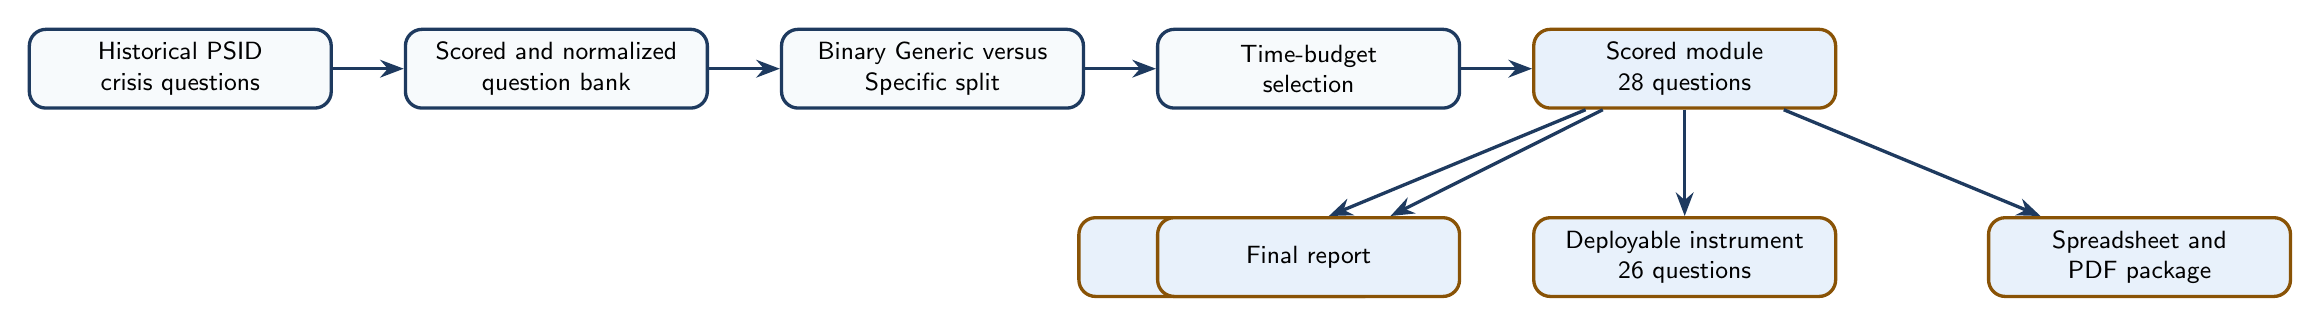
\begin{tikzpicture}[node distance=0.8cm and 0.9cm]
\node[flowstep] (a) {Historical PSID\\crisis questions};
\node[flowstep, right=of a] (b) {Scored and normalized\\question bank};
\node[flowstep, right=of b] (c) {Binary Generic versus\\Specific split};
\node[flowstep, right=of c] (d) {Time-budget\\selection};
\node[flowresult, right=of d] (e) {Scored module\\28 questions};
\node[flowresult, below=1.35cm of e] (f) {Deployable instrument\\26 questions};
\node[flowresult, below left=1.35cm and 1.9cm of e] (g) {Codebook};
\node[flowresult, below=1.35cm of d] (h) {Final report};
\node[flowresult, below right=1.35cm and 1.9cm of e] (i) {Spreadsheet and\\PDF package};
\draw[flowarrow] (a) -- (b);
\draw[flowarrow] (b) -- (c);
\draw[flowarrow] (c) -- (d);
\draw[flowarrow] (d) -- (e);
\draw[flowarrow] (e) -- (f);
\draw[flowarrow] (e) -- (g);
\draw[flowarrow] (e) -- (h);
\draw[flowarrow] (e) -- (i);
\end{tikzpicture}
}
\caption{Reporting flow from historical question bank to the current client bundle.}
\end{figure}

\section{What Changed in the Optimization Strategy}

\begin{table}[H]
\centering
\small
\begin{tabularx}{\textwidth}{L{0.19\textwidth} Y Y Y}
\toprule
Dimension & Legacy architecture view & Current production view & Why it changed \\
\midrule
Client-facing categories & Legacy architecture used 7 Generic Core rows, 1 Financial Crisis row, and 20 Pandemic / Disaster rows inside the older 28-row architecture & Current production uses 3 Generic and 25 Specific rows in the scored module, then 26 deployable rows after removing two demographic traceability items & The client package is easier to explain and the universal core is narrower and more portable. \\
Financial items & Finance appeared as its own visible label & Finance now competes inside Specific and is checked by redundancy penalties & Financial disruption remains covered without looking artificially dominant. \\
Deployment target & The scored shortlist was closer to the field-facing package & The scored shortlist is retained for traceability, while the field package is optimized separately for routine use & Separates analytic accountability from respondent burden. \\
Optimization levers & Ranking plus legacy toggle structure & Ranking plus portability bonus, construct coverage, redundancy control, documented wording replacements, and respondent-answer routing & The current package is optimized for a cleaner always-on instrument rather than for a broader archival architecture. \\
\bottomrule
\end{tabularx}
\caption{Before-versus-now view of the optimization strategy.}
\end{table}

\section{Methodology in Plain Language}

\subsection{How ranking works}

Each question receives a utility score for crisis relevance, a burden score for length and complexity, a baseline efficiency score $R_i$, and an augmented priority score $P_i$ that rewards distinctiveness and construct coverage.

\begin{psidbox}{Main formulae}
\begin{align*}
R_i &= \frac{U_i}{B_i} \\
B_i &= \max(0.10 \times \text{word\_count} + 0.20 \times \text{complexity}, 0.1) \\
P_i &= \frac{\text{augmented\_utility}}{B_i \times (1 + 0.65 \times \text{redundancy\_scaled})}
\end{align*}
\end{psidbox}

\subsection{How the binary category is assigned}

The client requested a simple threshold on $R_i$, but raw $R_i$ already exceeds 0.70 for the entire refreshed corpus. The workflow therefore applies the cutoff to normalized $R_i$ instead.

\begin{psidbox}{Operational thresholding}
\begin{align*}
\text{ri\_threshold\_score} &= \frac{R_i - \min(R_i)}{\max(R_i) - \min(R_i)} \\
\text{Generic} &\iff \text{ri\_threshold\_score} \geq 0.70 \\
\text{Specific} &\iff \text{ri\_threshold\_score} < 0.70
\end{align*}
\end{psidbox}

\subsection{How respondent answers now refine deployment}

\begin{table}[H]
\centering
\small
\begin{tabularx}{\textwidth}{L{0.22\textwidth} Y Y Y}
\toprule
Refinement source & What changes quantitatively & Why it helps & Assumption \\
\midrule
Generic-core answers and crisis identification & The effective interview path becomes the 3-item Generic core plus one crisis block; pandemic path is $1.40 + 2.92 = 4.32$ minutes, shutdown path is $1.40 + 4.20 = 5.60$, and disaster path is $1.40 + 20.30 = 21.70$ & Respondents are not forced through irrelevant blocks, so burden falls without changing the underlying row scores & One dominant crisis context is active for a standard administration. \\
Selected demographic traceability rows & Removing age and sex/gender reduces the routine deployable length by $1.167$ minutes & Keeps the instrument focused on direct crisis-impact content & Demographic context can be obtained elsewhere or only when needed. \\
Historical respondent distributions & Evidence on shutdown coping, stimulus use, and pandemic response justifies keeping aid, coping, and earnings-loss items salient & Grounds the optimization in observed behavior rather than only in wording similarity & Historical respondent patterns are informative for future crisis conditions. \\
Feed-forward respondent state & Prior-wave status, identity, address, and eligibility can refine follow-up universes without recalculating $U_i$, $B_i$, $R_i$, or $P_i$ & Preserves longitudinal logic while keeping the ranking stable and auditable & Prior-wave metadata is available when the module is deployed longitudinally. \\
\bottomrule
\end{tabularx}
\caption{Respondent-answer refinement changes the asked path, not the stored scoring fields.}
\end{table}

\section{Threshold Diagnostics}

\begin{table}[H]
\centering
\begin{tabularx}{\textwidth}{L{0.36\textwidth} R{0.12\textwidth} Y}
\toprule
Diagnostic & Value & Calculation / implication \\
\midrule
Minimum raw $R_i$ & 0.818 & $\min(R_i)$ across the refreshed corpus. \\
Maximum raw $R_i$ & 5.667 & $\max(R_i)$ across the refreshed corpus. \\
Rows with raw $R_i \geq 0.70$ & 52 of 52 & A raw threshold would classify every row as Generic. \\
Rows with normalized threshold score $\geq 0.70$ & 3 of 52 & Normalization creates the intended narrow portable core. \\
\bottomrule
\end{tabularx}
\caption{Why the Generic bucket is intentionally small after normalization.}
\end{table}

This is why the current \texttt{Generic} bucket contains only the most portable high-signal items after normalization.

\section{Selected Module Composition}

\begin{table}[H]
\centering
\footnotesize
\begin{tabularx}{\textwidth}{@{}L{0.14\textwidth} L{0.22\textwidth} R{0.11\textwidth} R{0.09\textwidth} R{0.10\textwidth} R{0.10\textwidth}@{}}
\toprule
Final category & Source & Selected questions & Minutes & Average $R_i$ & Average $P_i$ \\
\midrule
Generic & COVID-19 & 3 & 1.40 & 5.333 & 7.125 \\
Specific & Hurricane Katrina 2007 & 14 & 20.30 & 2.617 & 2.769 \\
Specific & COVID-19 & 5 & 2.92 & 3.364 & 4.393 \\
Specific & Govt Shutdown Income & 3 & 2.33 & 3.326 & 4.482 \\
Specific & Govt Shutdown Crisis & 1 & 1.87 & 3.719 & 4.592 \\
Specific & Understanding Society & 2 & 1.17 & 1.447 & 2.329 \\
\bottomrule
\end{tabularx}
\caption{Composition of the current scored module by final category and historical source.}
\end{table}

\section{Why Financial Questions Do Not Dominate the Final Module}

The earlier output looked more finance-heavy than the current one for two reasons. First, \texttt{Financial Crisis} used to appear as its own visible final label. Second, multiple finance-related items were close variants of one another, which made the previous structure look broader than it really was.

\begin{psidbox}{Interpretation}
\begin{itemize}
\item Financial items now compete within \texttt{Specific} instead of standing alone as a final category.
\item Redundancy penalties reduce the advantage of repeating near-identical income questions.
\item Katrina disaster items contribute many strong direct-exposure and trauma items.
\item The three highest-portability Generic items still capture crisis-related financial disruption without making finance the whole story.
\end{itemize}
\end{psidbox}

\section{Demographic Note}

\begin{table}[H]
\centering
\footnotesize
\begin{tabularx}{0.68\textwidth}{@{}L{0.34\textwidth} R{0.08\textwidth} R{0.10\textwidth} R{0.10\textwidth}@{}}
\toprule
Group & Rows & Average $R_i$ & Average $P_i$ \\
\midrule
Demographics only & 3 & 1.354 & 2.189 \\
Non-demographic crisis items & 49 & 2.253 & 2.584 \\
\bottomrule
\end{tabularx}
\caption{Demographic rows versus direct crisis-impact rows.}
\end{table}

\begin{itemize}
\item Demographic rows provide context and traceability.
\item They are not as efficient as direct crisis-impact questions for the deployable instrument.
\item That is why the final scored module can retain them while the deployable questionnaire removes them.
\end{itemize}

\section{Worked Example of a High-Value Generic Item}

Example question: \varname{GEN_LOSE_EARNINGS_PANDEMIC}

\begin{table}[H]
\centering
\begin{tabularx}{\textwidth}{L{0.18\textwidth} R{0.10\textwidth} Y Y}
\toprule
Field & Value & Calculation & Why it is used / assumption \\
\midrule
$U_i$ & 3.400 & $0.80 + 0.80 + 0.90 + 0.90$ & Utility aggregates the matched crisis-signal weights; assumes the keyword tags capture the item's substantive value. \\
$B_i$ & 0.600 & $\max(0.10 \times 6 + 0.20 \times 0.0, 0.1)$ & Burden converts wording cost into a penalty term. \\
$R_i$ & 5.667 & $3.40 / 0.60$ & Very high baseline signal per unit of burden. \\
$P_i$ & 7.860 & Value computed after rarity, construct, portability, and redundancy scaling & Strong augmented priority after distinctiveness adjustments. \\
minutes & 0.70 & $(6 \times 7) / 60$ & Short enough to retain in the universal core; assumes 7 seconds per word in oral administration. \\
Final category & Generic & $\text{ri\_threshold\_score} = 1.000 \geq 0.70$ & Portable across crisis types and strong enough to survive the binary threshold. \\
\bottomrule
\end{tabularx}
\caption{Characteristics of a high-value Generic item.}
\end{table}

This is the kind of item the new \texttt{Generic} bucket is meant to preserve: short, portable, and strongly informative.

\section{Conclusion}

The refreshed package is more disciplined than the earlier version in three ways:

\begin{itemize}
\item It keeps the category model easy to explain.
\item It preserves the quantitative ranking logic instead of replacing it with ad hoc pruning.
\item It separates the 28-row scored audit file from the 26-row deployable instrument, so burden reduction is explicit rather than hidden.
\item It cleanly separates technical documentation, deployable wording, and stakeholder reporting.
\end{itemize}

The result is a client package that is easier to defend analytically and easier to use operationally.

\end{document}